\chapter{Group by language groups}

\section{Language groups}
1 to 2, 3, 4, 5, etc. models on en-to-36 dataset (0.9 mil. sentences per target language)
compared with random runs
\subsection{Germanic group}

\begin{figure}[h]
	\begin{minipage}{0.48\textwidth}
	\centering
	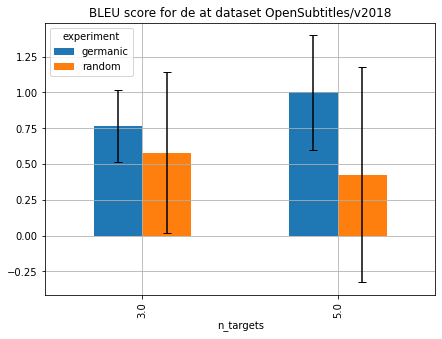
\includegraphics[width=0.9\columnwidth]{../img/de_opensubtitles_13_1.png}
	\end{minipage}\hfill
	%\vspace*{\floatsep}% https://tex.stackexchange.com/q/26521/5764
	\begin{minipage}{0.48\textwidth}
	\centering
	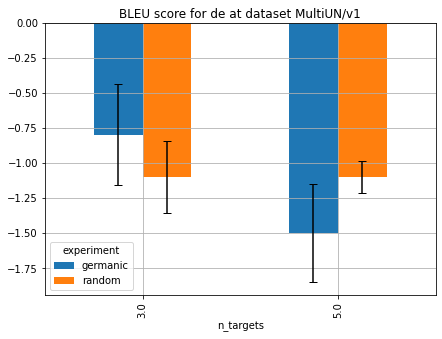
\includegraphics[width=0.9\columnwidth]{../img/de_multiun_25_4.png}
	\end{minipage}
	\mycaption{En\to{}De BLEU score difference: Random vs. Germanic}{
		On \emph{X} axis - number of target languages.
		On \emph{Y} axis - difference score comparing with monolingual BLEU.
		Left: OpenSubtitles/v2018, monolingual model's result 13.1 BLEU.
		Right: MultiUN, monolingual BLEU is 25.4.
	}
	\label{fig:de_random_vs_germanic}
\end{figure}

\begin{figure}[h]
	\begin{minipage}{0.48\textwidth}
	\centering
	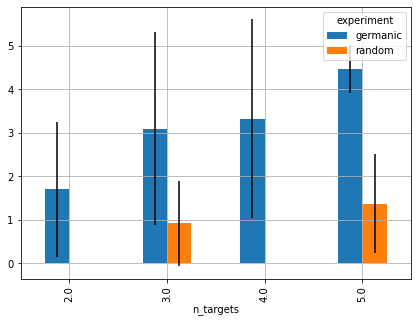
\includegraphics[width=0.9\columnwidth]{../img/da_opensubtitles_15_6.png}
	\end{minipage}\hfill
	\begin{minipage}{0.48\textwidth}
	\centering
	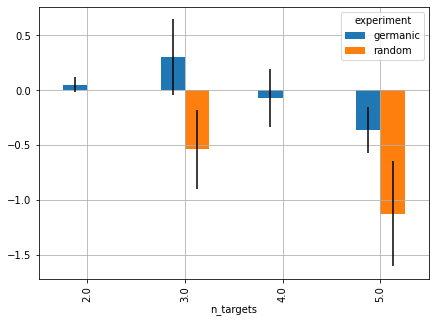
\includegraphics[width=0.9\columnwidth]{../img/da_europarl_24_6.png}
	\end{minipage}
	\mycaption{En\to{}Da BLEU score difference: Random vs. Germanic}{
		Axis are same as above.
		Left: OpenSubtitles/v2018, monolingual model's result 15.6 BLEU.
		Right: Europarl/v3, monolingual BLEU is 24.6.
	}
	\label{fig:da_random_vs_germanic}
\end{figure}



\subsection{Slavic with cyrillic script}

\begin{table}[h]
\begin{subtable}[t]{1\linewidth}
\begin{tabular}{rrrrrrr}
\toprule
n\_targets & \multicolumn{2}{l}{mean} & \multicolumn{2}{l}{count} & \multicolumn{2}{l}{std} \\
          &   cyrillic &   random & cyrillic & random &  cyrillic &    random \\
\midrule
        2 &  14.950000 &  15.2625 &      6.0 &    8.0 &  1.209545 &  0.757699 \\
        3 &  15.383333 &  14.5625 &      6.0 &    8.0 &  0.725029 &  0.616297 \\
        4 &  15.200000 &  14.2750 &      2.0 &    4.0 &  0.282843 &  0.206155 \\
\bottomrule
\end{tabular}
\caption{MultiUN/v1}
\label{table:ru/multi_un}
\end{subtable}
\begin{subtable}[t]{1\linewidth}
\begin{tabular}{rrrrrrr}
\toprule
n\_targets & \multicolumn{2}{l}{mean} & \multicolumn{2}{l}{count} & \multicolumn{2}{l}{std} \\
          &   cyrillic &  random & cyrillic & random &  cyrillic &    random \\
\midrule
        2 &  22.883333 &  22.875 &      6.0 &    8.0 &  0.507609 &  0.514782 \\
        3 &  22.333333 &  21.050 &      6.0 &    8.0 &  0.273252 &  0.705084 \\
        4 &  21.050000 &  20.950 &      2.0 &    4.0 &  0.494975 &  0.465475 \\
\bottomrule
\end{tabular}
\caption{NewsCommentary/v11}
\label{table:ru/news_v11}
\end{subtable}
\begin{subtable}[t]{1\linewidth}
\begin{tabular}{rrrrrrr}
\toprule
n\_targets & \multicolumn{2}{l}{mean} & \multicolumn{2}{l}{count} & \multicolumn{2}{l}{std} \\
          &   cyrillic &   random & cyrillic & random &  cyrillic &    random \\
\midrule
        2 &  19.266667 &  18.7375 &      6.0 &    8.0 &  0.273252 &  0.396187 \\
        3 &  19.350000 &  17.7875 &      6.0 &    8.0 &  0.653452 &  0.418970 \\
        4 &  18.900000 &  17.5750 &      2.0 &    4.0 &  0.282843 &  0.613052 \\
\bottomrule
\end{tabular}
\caption{OpenSubtitles/v2018}
\label{table:ru/news_v11}
\end{subtable}
\caption{Mean BLEU score, its standard deviation and number of trained models (count) for Russian at various datasets}
\end{table}



\begin{table}[h]
\begin{subtable}[t]{1\linewidth}
\begin{tabular}{rrrrrrr}
\toprule
n\_targets & \multicolumn{2}{l}{mean} & \multicolumn{2}{l}{len} & \multicolumn{2}{l}{std} \\
          &   cyrillic &     random & cyrillic & random &  cyrillic &    random \\
\midrule
        2 &  40.433333 &  40.683333 &      6.0 &    6.0 &  0.273252 &  0.183485 \\
        3 &  39.216667 &  39.506250 &      6.0 &   16.0 &  0.318852 &  0.611521 \\
        4 &  37.750000 &  39.450000 &      2.0 &    4.0 &  0.494975 &  0.525991 \\
        5 &        NaN &  38.483333 &      NaN &   12.0 &       NaN &  0.511386 \\
\bottomrule
\end{tabular}
\caption{Europarl/v7}
\label{ table:bg/Europarl/v7 }
\end{subtable}
\begin{subtable}[t]{1\linewidth}
\begin{tabular}{rrrrrrr}
\toprule
n\_targets & \multicolumn{2}{l}{mean} & \multicolumn{2}{l}{len} & \multicolumn{2}{l}{std} \\
          &   cyrillic &     random & cyrillic & random &  cyrillic &    random \\
\midrule
        2 &  23.683333 &  23.250000 &      6.0 &    6.0 &  0.598052 &  0.225832 \\
        3 &  23.216667 &  22.406250 &      6.0 &   16.0 &  0.470815 &  0.619106 \\
        4 &  22.300000 &  22.600000 &      2.0 &    4.0 &  0.424264 &  0.081650 \\
        5 &          - &  21.741667 &        - &   12.0 &         - &  0.494439 \\
\bottomrule
\end{tabular}
\caption{OpenSubtitles/v2018}
\label{tab:bg/OpenSubtitles/v2018}
\end{subtable}
\caption{BLEU score for Bulgarian at various datasets }
\end{table}

\begin{table}[]
\begin{tabular}{r|rr|cc|rr}
\toprule
n\_targets & \multicolumn{2}{c}{mean} & \multicolumn{2}{c}{count} &\multicolumn{2}{c}{std} \\
          &   cyrillic &  random & cyrillic & random &  cyrillic &    random \\
\midrule
        1 & \multicolumn{2}{c|}{41.40} & \multicolumn{2}{c|}{1} & \multicolumn{2}{c}{-}  \\
\midrule
        2 &         40.30 &      40.60 &           3 &        3 &       0.17 &      0.20 \\
        3 &         38.97 &      39.39 &           3 &        8 &       0.23 &      0.62 \\
        4 &         37.40 &      39.40 &           1 &        2 &        --  &      0.71 \\
        5 &           --  &      38.45 &         --  &        6 &        --  &      0.52 \\
\bottomrule
\end{tabular}

\caption{BLEU score for  bg at dataset Europarl/v7 }
\label{ table:bg/Europarl/v7 }
\end{table}
\section{Selecting target languages by linguistic similarity}

